%*----------- SLIDE -------------------------------------------------------------
\begin{frame}[t]{Introdução} 
    \framesubtitle{Planejador global}
    O planejador de trajetória global tem como objetivo encontrar um caminho entre duas localizações em um mapa global.

    Planejadores globais aderentes ao nav core::BaseGlobalPlanner:
    %\newline
        \begin{columns}[t]
            \column{.05\linewidth}
            \column{.4\linewidth}
                \begin{enumerate}
                    \item Global planner
                    \item Navfn
                    \item Carrot planner
                \end{enumerate}
            \column{.6\linewidth}
            \begin{center}
            %\centerline{
                \begin{figure}
                    %
\includegraphics[width=1\textwidth]{pista}
                    % \caption{Pista de corrida \cite{agostini2007}}
                    \roundpic[xshift=-0.7cm,yshift=0.5cm]{2.5cm}{6cm}{trajetoria}
                    %\caption{Pista de corrida \cite{agostini2007}}
                \end{figure}
            %}
            \end{center}
        \end{columns}
        \vspace*{0.6cm}
        Há a possibilidade de inserir plugins com outros métodos de planejamento global.
%*----------- notes
    \note[item]{Notes can help you to remember important information. Turn on the notes option.}
\end{frame}
%-
%*----------- SLIDE -------------------------------------------------------------
\begin{frame}[t]{D*}
    \framesubtitle{Classificações}
    % \begin{columns}
    %     \column{.1\textwidth}
    %     \column{.4\textwidth}
    %     \column{.4\textwidth}
    % \end{columns}

    \begin{block}{D* original}
        -Nome baseado no termo "Dinâmico A*"\\
        -Desenvolvido por Anthony Stentz
    \end{block}

    \begin{alertblock}{D* focalizado}
        -Combina ideias do A* e do D* original\\
        -Desenvolvido por Anthony Stentz
    \end{alertblock}

    \begin{exampleblock}{D* lite}
        -Baseado no Lifelong Planning A*\\
        -Desenvolvido por Sven Koenig e Maxim Likhachev 
    \end{exampleblock}
 %*----------- notes
    \note[item]{Notes can help you to remember important information. Turn on the notes option.}
\end{frame}
%-
%*----------- SLIDE -------------------------------------------------------------
\begin{frame}[t]{D*}
    \framesubtitle{Funcionamento}
    \begin{enumerate}
        \item Os algoritmos de busca D* resolvem os problemas de planejamento baseados em suposições
        \item Novas informações são adicionadas ao mapa e se necessário uma nova trajetória é planejada
        \item Os sistemas atuais são normalmente baseados no D* lite
    \end{enumerate}

    \begin{figure}
        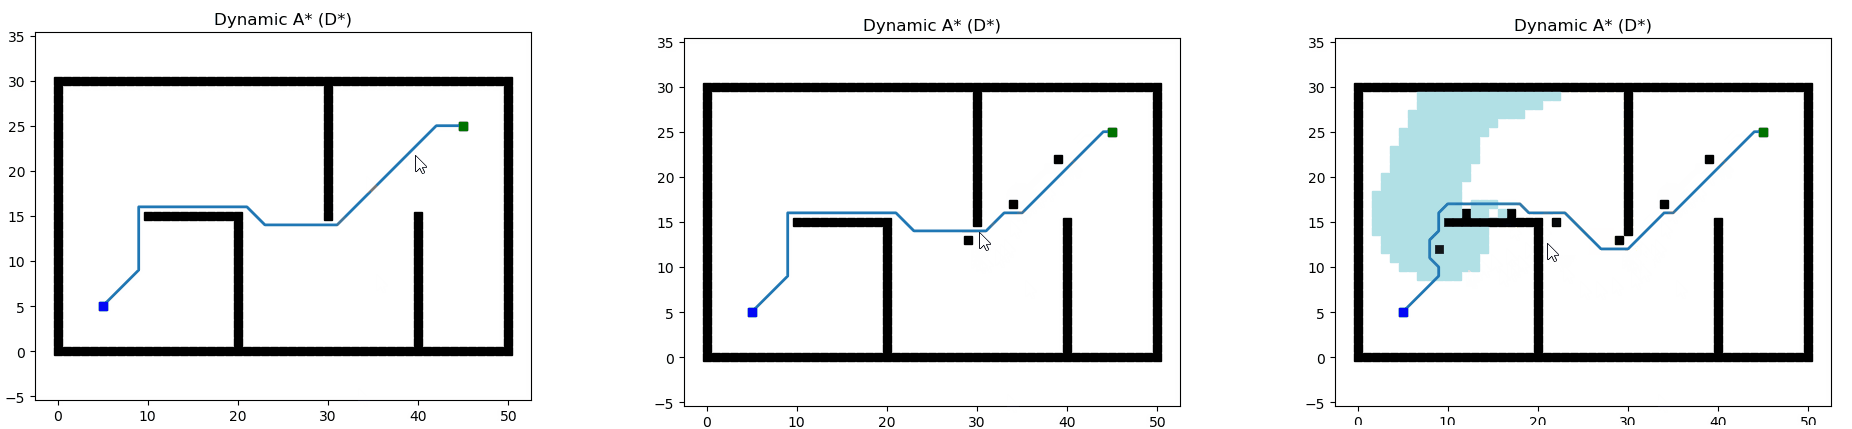
\includegraphics[trim = 0 20 0 50, clip, width=0.8\textwidth]{funcionamento.png}
        %\caption{.}
    \end{figure}
%*----------- notes
    \note[item]{Notes can help you to remember important information. Turn on the notes option.}
\end{frame}
%-
%*----------- SLIDE -------------------------------------------------------------
\begin{frame}[c]{Metodologia}
    \begin{figure}
        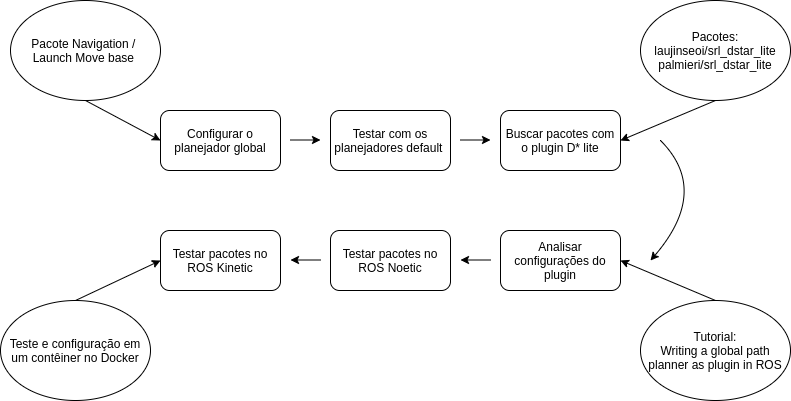
\includegraphics[width=0.8\textwidth]{metodologia.png}
        %\caption{.}
    \end{figure}
%*----------- notes
    \note[item]{Notes can help you to remember important information. Turn on the notes option.}
\end{frame}
%-
%*----------- SLIDE -------------------------------------------------------------
\begin{frame}[c]{Considerações Finais}
    \begin{columns}
        \column{.00\textwidth}
        \column{.5\textwidth}
            \begin{itemize}
                \item Gera uma trajetória global
                \item Dificuldade para gerar a trajetória
                \item Dificuldade para atualizar a trajetória
                \item Bons resultados em curtas distâncias
            \end{itemize}
        \column{.5\textwidth}
             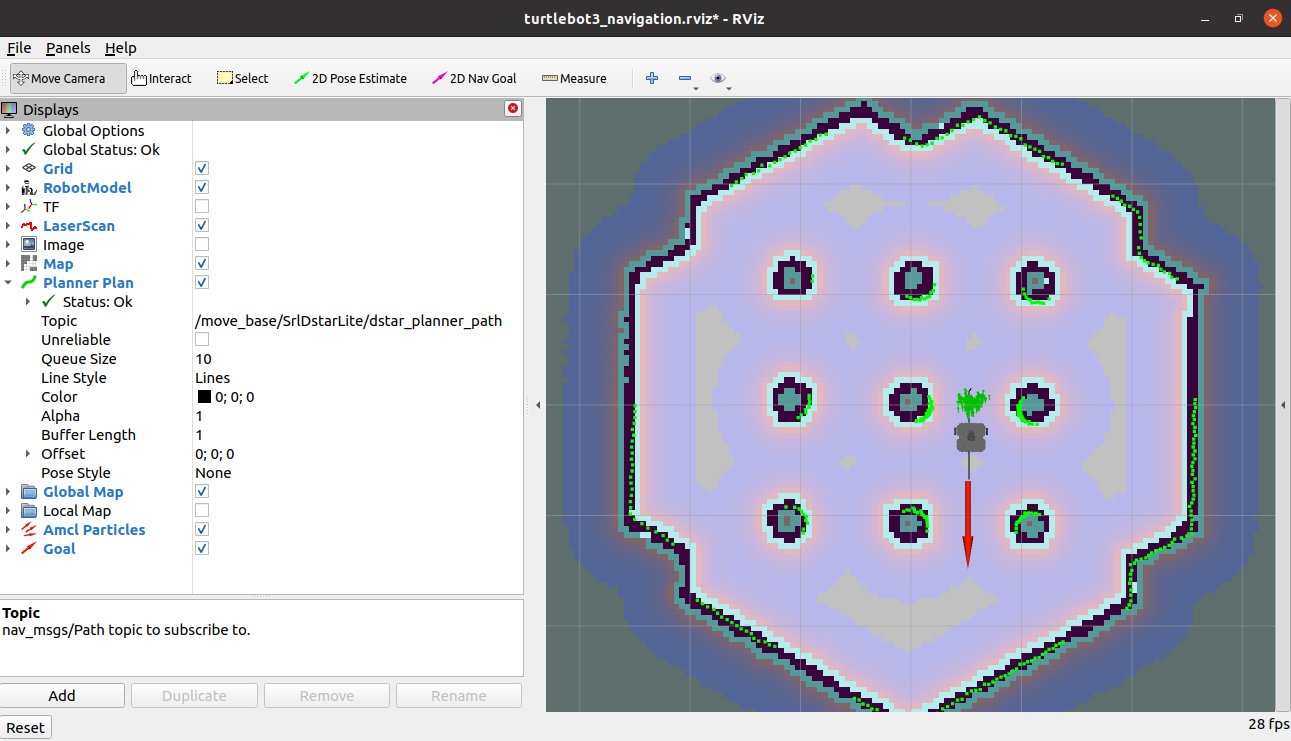
\includegraphics[width=\textwidth]{result.png}
    \end{columns}
 %*----------- notes
    \note[item]{Notes can help you to remember important information. Turn on the notes option.}
\end{frame}
%-